\begin{figure}[ht]
  \caption{Average TVP prices for different consumption profiles}\label{fig:marschak}
  \begin{center}
  {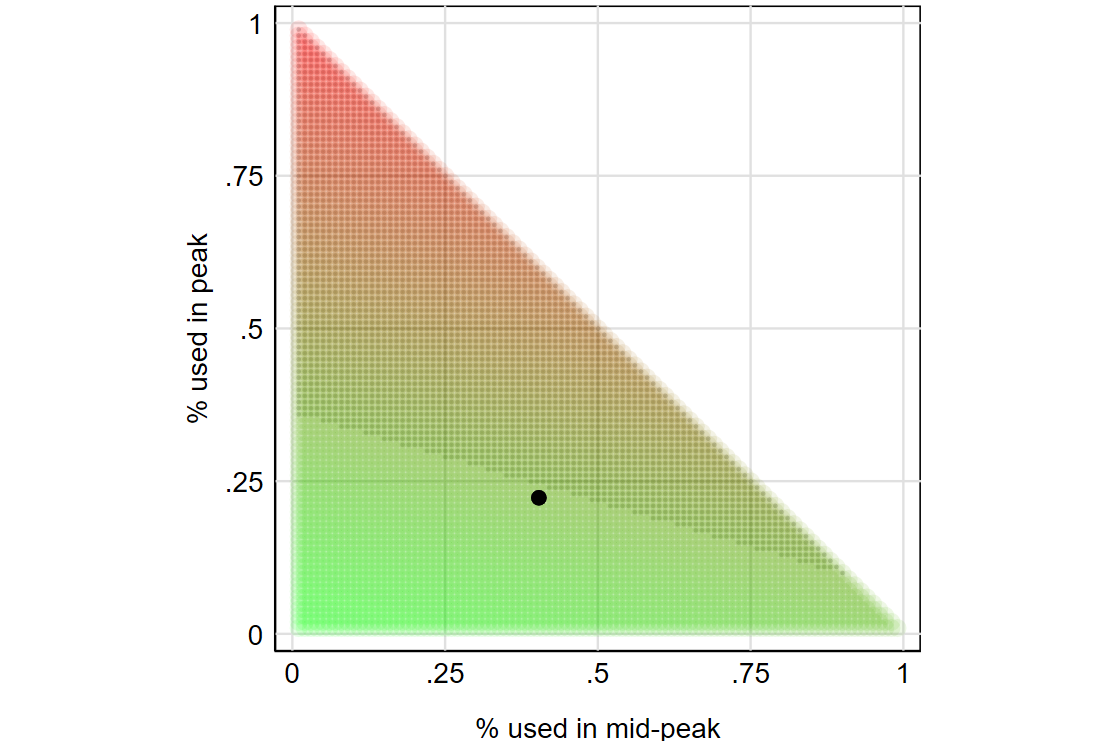
\includegraphics[width=1\textwidth]{./figures/marschak.png}}
  \end{center}
  \fnote{}
\end{figure}

In Figure \ref{fig:marschak} we use a Marschak-Machina triangle to show all possible consumption profiles. The average price a consumer pays for electricity under TVP depends on the share of consumption in each of the three relevant periods (peak, mid-peak, and off-peak). The y-axis in the figure represents the share of consumption during peak hours ($p$), the $x$-axis represents the share of consumption during mid-peak hours ($m$), and the residual $1-p-m$ represents the share of consumption during off-peak hours. For example, the $xy$-coordinate $(0.40,0.22)$, marked by a black dot, represents the average consumption profile of households in the TVP of our study. On average the share of electricity used in peak, mid-peak, and off-peak hours is 22\%, 40\%, and 38\%. The shaded area (top of the figure) shows all the consumption profiles in which the average price under block pricing is higher than the average price under TVP. Further, the color green at the bottom of the graph (and its intensity) indicates low average prices under TVP and the color red at the top of the graph (and its intensity) indicate high average prices under TVP. \footnote{To make this graph we used the actual prices from our study, both under block pricing and under TVP. We normalized total consumption to 100 and calculated the price a household would pay under block pricing (i.e., a constant price based on the total consumption) and the price a household would pay under TVP under all possible consumption profiles (i.e., the price changes depending on when the household uses the electricity).}

From Figure \ref{fig:marschak} we learn that (i) the average pricing under TVP is not always lower than the average price under block pricing, (ii) there is significant variation in the average price a household would pay under TVP depending on their consumption profile, and (iii) households from our study have an average consumption profile for which the average price under TVP is lower than the average price under block pricing. As discussed in the introduction, we believe that because the TVP program is voluntary (as most TVP programs around the world), the location of the black dot in the non-shaded area (where TVP price $<$ block price) is likely because of self-selection on future gains. In other words, we expect the first households to voluntary join a TVP program to be precisely the households that stand to gain the most. It is still an open question, however, whether these households stand to gain because their consumption profile was already in the non-shaded area or because these households were able to adjust their consumption.\footnote{Analyzing this would require better data to observe consumption during the day before and after the TVP program. We do not have this data, and it is extremely difficult to acquire or rare to find such data in settings we study.}

\FloatBarrier
